\subsection{Controlled execution studies}
\label{sec:supplement}
The following studies distinguish stored-topology execution, differentiated
message computation and first-call cost from the dynamic-search comparisons.
They use the same single-GPU host, with three fresh processes per configuration,
seeds 20260921--20260923, four warmups and ten checked calls per process.
Configuration order is randomized. Plots show the median and range of process
medians, not a confidence interval. Feature values alternate between two
snapshots; the input copy and checking are outside the synchronized wall timer.
Reported memory is peak Torch-allocated storage, including live topology,
inputs, outputs, tapes and workspaces, but excluding allocator reserve, CUDA
context and other processes. The source snapshot is independent of the older
experiments; unchanged hardware does not imply an unchanged implementation.

\paragraph{Holding topology constant.}
A common radius search produces a fixed CSR snapshot at 8,192 or 32,768
uniform binary-grid points, with nominal degree 32. The three consumers receive
identical indices, Euclidean weights and 32- or 128-component features: Tiga's
compiled weighted sum, Torch gather--multiply--scatter, and Torch sparse matrix
multiplication. Search is outside timing for all three. CSR hashes are checked
between peers in each trial. This is a topology-controlled execution-path
comparison, not a single-pass on/off ablation: traversal, dispatch and reduction
strategy can still differ.

\begin{figure}[htbp]
\centering
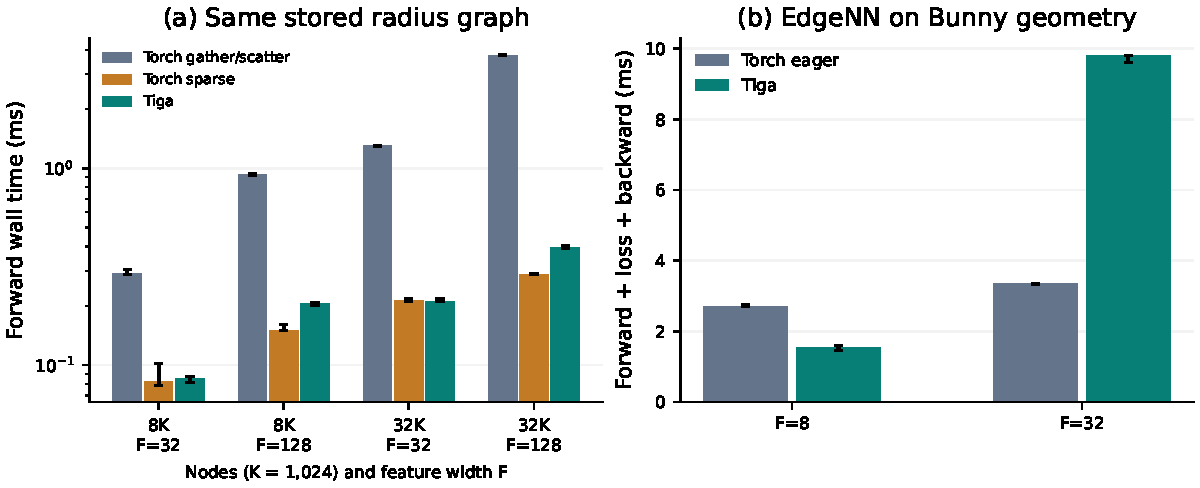
\includegraphics[width=\linewidth]{figures/supplement-execution.pdf}
\caption{Supplementary execution studies. (a) The same stored radius topology
is consumed by three implementations; graph construction is excluded.
(b) Differentiated EdgeNN steps on a radius graph of Stanford Bunny geometry.
Bars show medians of three process medians, with their ranges. Lower is better;
only panel (a) uses a logarithmic axis.}
\label{fig:supplement}
\end{figure}

At 32,768 nodes and 128 features, measured forward times are 0.395 ms, 3.759 ms, 0.289 ms for Tiga, Torch gather/scatter and Torch sparse, respectively. Median process-peak allocations are 67.3 MiB, 1007.3 MiB, 67.6 MiB. These measurements hold search and topology fixed; execution strategy and launch overhead still differ.

The reduction in intermediate storage is clear against explicit message
materialization; the optimized sparse-library peer can be faster than Tiga
and has similar storage. Thus eliminating edge messages is useful but does
not alone establish a better schedule than a sparse library. This study does
not isolate the separate gain from avoiding accepted-edge storage in the
generated-radius experiment.

\paragraph{Differentiation on real geometry.}
The Stanford Bunny zippered reconstruction provides 35,947 reconstructed
vertices~\cite{stanfordbunny}. Coordinates are centered and divided by the largest
bounding-box extent; radius 0.015 gives 356,260 directed non-self edges. The
reconstructed surface is the data source, not raw scanner noise. Features are
synthetic; an untrained MLP maps displacement and source features through a
32-unit ReLU layer to three outputs, summed at destinations. The mean squared
difference from normalized positions supplies a scalar regression loss.
Both paths use the same fixed graph and parameters. This workload measures a
differentiated geometric operator, not downstream task accuracy, convergence
or a complete optimizer step.

Every retained call checks outputs and gradients of features, positions and
all four parameter tensors against explicit Torch gather--MLP--scatter.
Position gradients hold edge membership fixed. In addition to elementwise
tolerances, each gradient must have relative L2 error below 0.002. The Tiga
path must report its compiled tile VJP; a reference fallback is rejected.
Table~\ref{tab:supplement-edgenn} separates forward from loss-plus-backward.
Independent medians of these stages need not sum exactly to the median total.

\begin{table}[htbp]
\centering\small
\begin{tabular}{llrrrr}
\toprule
Input width & Path & Forward (ms) & Backward (ms) & Total (ms) & Peak (MiB) \\
\midrule
8 & Torch eager & 0.64 & 2.07 & 2.71 & 172.25 \\
8 & Tiga & 0.86 & 0.72 & 1.54 & 32.34 \\
32 & Torch eager & 0.94 & 2.42 & 3.36 & 209.22 \\
32 & Tiga & 0.92 & 8.86 & 9.79 & 37.58 \\
\bottomrule
\end{tabular}

\caption{Bunny EdgeNN: medians across three process medians. Peak allocation is
the median of per-process measured peaks. Backward includes loss construction;
no optimizer update is timed.}
\label{tab:supplement-edgenn}
\end{table}

At width eight, the measured total improves from 2.71 to 1.54 ms with substantially
less allocated storage. At width 32, Tiga uses less storage but its 8.86 ms
backward makes the total slower than Torch. Recompute-based fusion is therefore
a memory--time tradeoff, not a universal training acceleration. This experiment
does not independently isolate recomputation, atomic accumulation and scheduling
as causes of that slowdown.

\paragraph{First result and amortization.}
For the 32,768-node, 32-feature stored-radius case, three additional worker pairs
use empty isolated Triton, TorchInductor and CUDA caches, then reuse each pair's
disk caches in a new process. Imports, CUDA initialization, graph setup and the
eager correctness oracle precede timing. The first result includes Tiga capture,
lowering, provider work, module loading and execution, rather than pure compile
time. A disk-cache hit does not restore an in-process executable.
The gather/scatter peer has already served as the correctness oracle, so its
entry is the first timed call, not cold library initialization. All entries
exclude that common setup; this is an execution-ready comparison rather than
time from launching Python to a first answer.

\begin{table}[htbp]
\centering\small
\begin{tabular}{lrr}
\toprule
Path & First result (ms) & Warm call (ms) \\
\midrule
Tiga, empty isolated caches & 1105.5 (1095.5--1113.8) & 0.214 \\
Tiga, reused disk caches & 635.1 (621.9--651.4) & 0.216 \\
Torch sparse, fresh process & 17.0 (16.9--17.5) & 0.213 \\
Torch gather/scatter, fresh process & 1.3 (1.2--1.3) & 1.301 \\
\bottomrule
\end{tabular}

\caption{First-result cost versus warm execution. First-result entries show
median and range of three fresh processes; warm entries are medians of process
medians. Common setup is excluded; the gather/scatter oracle is already warm.
Torch sparse uses its ordinary library environment.}
\label{tab:supplement-jit}
\end{table}

For first-result cost $C$, warm time $t$ and $K$ calls, an amortization model is
$$
T(K)=C+(K-1)t.
$$
The model assumes stable warm time; it is not a measured cumulative-time curve.
Here the cold first result costs about 1.11 s, and persistent-cache reuse still
costs about 0.64 s. Warm Tiga and Torch sparse are both about 0.21 ms, with no
measured steady-state advantage supporting an amortized crossover against the
sparse peer. Against explicit gather/scatter, warm savings can amortize setup
over repeated calls.
Using the reported medians, the model predicts a crossover against explicit Torch gather/scatter after approximately 1,018 calls. This is a model-derived estimate, not an observed crossover.

Short-lived programs should not be assigned warm-kernel
speedups without this qualification.
\FloatBarrier
